% !TeX root=../../../main.tex

\chapter{روش‌های پیشین}
% دستور زیر باعث عدم‌نمایش شماره صفحه در اولین صفحهٔ این فصل می‌شود.
%\thispagestyle{empty}

\section{مقدمه}
در فصل گذشته به معرفی مفاهیم و موضوعات مرتبط با این حوزه پرداخته شد. در ادامه در این فصل با توجه به اطلاعاتی که کسب کرده‌اید به معرفی و بررسی روش‌هایی که مرتبط با موضوع این پایان‌نامه است پرداخته خواهد شد و نتایج آن‌ها را برای فرض‌های و داده‌های ورودی خود مشاهده خواهیم نمود. در این بین تا جایی که ممکن باشد به بررسی نقاط قوت و ضعف آن‌ها نیز خواهیم پرداخت و در انتهای این فصل یک جدول مقایسه بین روش‌هایی که تا به حال معرفی شده‌اند را ارائه خواهیم داد.

%در ابتدای این فصل به معرفی مقاله و روش SCITE خواهیم پرداخت که البته یکی از مقالات اصلی پایان‌نامه جاری می‌باشد و یکی از روش‌های پیشنهادی در فصل آینده نیز بر پایه همین روش می‌باشد.


\section{\gls{tumorevolutionarytreeinference} با استفاده از داده‌های \gls{scs}}
\gls{cancer} نامی است که به مجموعه¬ای از بیماری¬ها اطلاق می¬شود که از تکثیر مهار نشده سلول¬ها پدید می¬آیند. تحقیقات انجام شده نشان می¬دهد که سرطان در واقع یک فرآیند تکاملی از جهش¬های  ژنتیکی، شامل حذف و تغییر تعداد کپی ، حذف و تغییر تک نوکلئوتیدد¬ها  ، بازسازی و جایگزینی ژن¬ها در سلول¬های توموری است. در واقع تومور زمانی ایجاد می¬شود که یک سلول جهش یافته بتواند با عبور از سیستم دفاعی بدن زندگی کرده و تکثیر شود به گونه¬ای که نسبت مرگ به تولید آن گونه ایجاد شده بسیار کوچک تر از 1   ($\alpha \ll 1$) باشد. با پیشرفت تومور، ناهنجاری¬های ژنتیکی  مختلف منجر به افزایش گروه¬های جمعیتی ناهمگنی به نام کلون  می¬شود. فرآیند تکاملی همه این کلون¬ها را می¬توان با یک درخت فیلوژنی   و آنالیز فیلوژنیتیکی از چندین کلون سلولی سرطانی مدل¬سازی کرد که می¬تواند مطالعه انواع تومور را تسهیل کند. ساختار و الگو¬های درون این درخت میزان وابستگی بین گونه¬های خاص را با توجه به تعداد و فواصل بین اجداد مشترک¬شان تعیین می¬کند. درخت¬های فیلوژنی عملکرد بارزی در توصیف فرآیند توسعه تومور دارند که بهتر از دیگر الگوریتم¬های مشابه عمل می¬کنند. تحلیل توپولوژی درخت درخت پیشرفت تومور نشان می¬دهد که مسیر توسعه تومور در طول مراحل مختلف تشکیل تومور، تا حد زیادی تغییر می¬کند و البته نتایج مبتنی بر درخت بهتر از نتایج داده¬های بدست آمده از طریق روش¬های دیگر در تشخیص تومور می¬باشد.
در حال حاضر ظهور تکنولوژی¬های بر پایه \gls{dna} یک سلول منفرد ، با هدف افزایش دانش از جنبه¬های مختلف بیولوژی سرطان، شامل بررسی زیرساخت کلونال، ردیابی تکامل تومور، شناسایی زیرکلون¬های نادر و درک ریزمحیط-های سرطانی در پیشرفت تومور، به یاری محققان این حوزه آمده و بالاترین وضوح را از تاریخچه سرطان (درخت فیلوژنی) فراهم کرده است. در واقع از آنجایی که در روش¬ توالی¬یابی تک سلولی  گونه¬های مختلف از ابتدا از هم جدا  می¬شوند، از نقطه منظر از دست دادن تنوع در زیرجمعیت بافت مورد آزمایش نداریم و به همین دلیل دقت این روش نیز نسبت به روش انبوه بالاتر می¬باشد. در کنار مزایا این روش، معایبی چون، هزینه بالا، از دست دادن سلول¬ها، جهش ثانویه در هنگام کشت، از دست دادن میزان فراوانی درون تومور حقیقی و زمان¬گیر بودن فرآیند نمونه گیری اشاره کرد.

در ابتدا استفاده از روش¬های توالی¬یابی انبوه  بدلیل اینکه حجم بالایی از اطلاعات در اثر این توالی¬یابی ایجاد می¬شود، از محبوبیت بیشتری برخوردار بود  اما با پیشرفت تکنولوژی و ظهور روش¬های نوینی چون توالی¬یابی تک¬سلولی این مهم دچار تغییر شد. در روش توالی¬یابی انبوه، نمونه¬برداری بر روی تعداد بسیار زیادی سلول ( از محدوده¬ی هزار تا میلیون سلول) صورت می¬گرفت و حجم بالای داده¬ها و امکان تفکیک پایین نواحی ناهمگن، اطلاعات کافی از ساختار درون تومور و ناهمگنی¬های درون توموری بدست نمی¬داد. در مقابل، در روش توالی¬یابی تک¬سلولی، اگر¬چه میزان هزینه نمونه¬برداری افزایش قابل¬توجهی داشت و یا میزان اطلاعات از دست رفته  و نویز موجود در داده¬های توالی¬یافته بالا بود\cite{deshwar2015phylowgs, dean2001rapid}.


اما در این روش رزولوشن یا قدرت تفکیک جهش¬های گوناگون از یکدیگر بسیار بالا بود و تشخیص نواحی ناهمگنی تومور و تفکیک زیرکلون¬ها از یکدیگر بسیار راحت¬تر از گذشته صورت می¬گرفت. در این فصل روش¬هایی را مورد بررسی قرار می¬دهیم که ساخت درخت فیلوژنی تومور و ناهمگنی¬های درون توموری را از طریق داده¬های توالی¬یابی تک¬سلولی مورد بررسی قرار می¬دهد.


\subsection{مدل کیم و سایمون\cite{kim2014using}} 

این مدل در سال 2014 با تمرکز بر ساخت \gls{phylogenytree}  از طریق رابطه ترکیبی میان جهش¬های ایجاد شده در داده-های توالی¬یابی تک¬سلولی \gls{dna} ارائه گردید. بررسی رابطه¬ی ترتیبی هر یک از جهش¬های رخ داده با یکدیگر، این امکان را فراهم می¬آورد تا اطلاعاتی در مورد نحوه تشکیل کلون¬ها و ترتیب زمانی رخ دادن جهش¬های گوناگون بدست آید. همچنین امکان محاسبه نسبت زمانی سپری شده میان جهش¬های اولیه موجود در داده¬های توالی¬یابی تک¬سلولی تا نزدیک¬ترین جد مشترک وجود دارد. استنباط \gls{phylogenytree} از طریق لگوریتم کیم و سایمون، بر مبنای منطق بیزی است، یعنی از این منطق به منظور تعیین رابطه ترتیبی بین هر دو جهش گوناگون استفاده شده است. در ادامه مقدار بیشینه درستنمایی درخت استنباط شده بر مبنای احتمال ترتیبی دوبه¬دوی بین هر دو جهش مختلف در دو جایگاه از یک دنباله، که از طریق ژنولوژی متفاوت با جهش¬های گوناگون در گره¬های درخت به هم مرتبط می¬شوند، محاسبه می¬شود. سرانجام مقادیر بیشینه¬ی  احتمالات با شرط کمینه کردن میزان تفاوت با داده¬های مشاهده شده محاسبه می¬گردد. 

از نکات قوت این الگوریتم در نظر گرفتن خطای توالی¬یابی و  \gls{alleledropout} است. این عدم قطعیت در داده¬ها از طریق محاسبه ماکزیمم درست¬نمایی ترتیبی هر یک از جهش¬ها بدست خواهد آمد. به عنوان مثال در نظر بگیرید که هفت زوج مرتب از جهش¬های یک \gls{dna} موجود است. برای سادگی بیشتر مولفه اول را  با \lr{x} و مولفه دوم را با \lr{y} نشان داده¬ می¬شود. داده¬های نمونه¬¬گیری شده از این \gls{dna}  در جدول زیر نشان داده شده¬است:

\begin{center}
\begin{tabular}{|l|l|l|l|l|l|l|l|}
	\hline
	\lr{Sample}&$1$&$2$&$3$&$4$&$5$&$6$&$7$\\\hline
	\lr{X mutation}&$0$&$0$&$0$&$0$&$1$&$1$&$0$\\\hline
	\lr{Y mutation}&$0$&$0$&$1$&$1$&$1$&$1$&$1$\\\hline
\end{tabular}
\end{center}



در این جدول صفر بیانگر عدم وجود جهش و یک بیانگر وجود جهش است. تعداد رخداد جهش¬ها با فرض عدم وجود خطا در توالی¬یابی داده¬ها، برابر یک در نظر گرفته می¬شود، یعنی در هر موقعیت تنها یکبار جهش رخ داده است. همچنین ترتیب زمانی رخداد جهش¬ها یک ترتیب جزئی است، به این معنی که زوج (1,1) بیانگر این است که یا جهش \lr{x} مقدم بوده است یا جهش \lr{y}. زوج (0,1) بیانگر آن است که جهش \lr{x} وجود نداشته است ولی جهش \lr{y} وجود داشته و با فرض اینکه هیچ جهشی از بین نمی¬رود، در نتیجه می¬توان استنباط کرد که \lr{y} نسبت به x قدیمی¬تر است و به عنوان یکی از اجداد \lr{x} در \gls{phylogenytree} تومور قرار می¬گیرد. در نتیجه با استفاده از جدول داده¬های نمونه¬برداری شده، استنباط یک رابطه زمانی میان جهش¬های صورت گرفته امکان پذیر است. شکل \ref{fig:ch_rw:intro_phylo} یک درخت فیلوژنیک تومور را نشان می¬دهد که از داده¬های جدول بالا استنباط شده است. در این همه هفت نمونه به عنوان برگ¬های درخت مشاهده می¬شود و ریشه درخت زوج (0,0) می¬باشد به این معنی که در ابتدا هیچ جهشی رخ نداده است. محور عمودی بیانگر سیر زمانی تکامل تومور است که به تعداد نمونه¬ها تقسیم شده است. 


\begin{figure}[!ht]
	\centerline{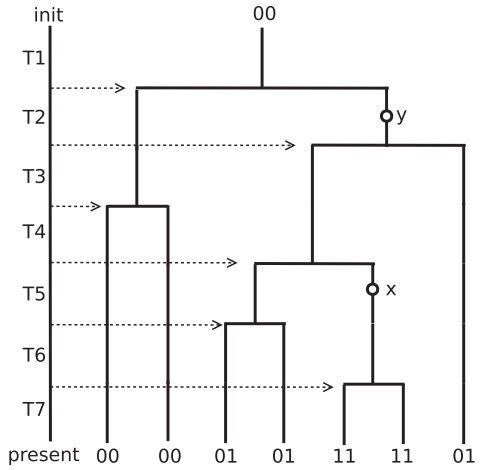
\includegraphics[width=10cm]{chaps/rw/intro_phylo}}
	\caption{عنوانننننننننننننننننننننننن}
	\label{fig:ch_rw:intro_phylo}
\end{figure}

برای استنباط درخت فیلوژنی تومور، الگوریتم کیم وسایمون از سه بخش اصلی تشکیل شده است. طبق قضیه بیز برای محاسبه هر یک از این سه احتمال به مقادیر \gls{likelihood}  نیاز داریم. مقدار احتمال رخداد طبق رابطه¬ زیر محاسبه می¬گردد:

\begin{center}
	\begin{math}
		P(x) = yyyyyyyyyyyyyyyyyyyyyyyyyyyy
	\end{math}
\end{center}

طبق این رابطه و با توجه به اینکه رابطه¬ زمانی میان جهش¬های \lr{x} و \lr{y} دارای 3 حالت 
\begin{center}
	\lr{$x \rightarrow y$} ، \lr{$y \rightarrow x$}  و  \lr{$x \not\leftrightarrow y$}
\end{center}
است، مقدار احتمال محاسبه شده از رابطه فوق به ازای یکی از این سه حالت بیشینه است و به ازای آن حالت یک مسیر جهت¬دار در درخت فیلوژنی قرار خواهد گرفت. طبق آنچه گفته شد یک گرف جهت دار فیلوژنی بلقوه مشابه آنچه در شکل زیر نشان داده ¬شده است استنباط خواهد شد. در نهایت از این گراف جهت دار، یک درخت به طوری که روابط میان جهش¬ها از آن استنباط شود ساخته خواهد شد. 

\begin{figure}[!ht]
	\centerline{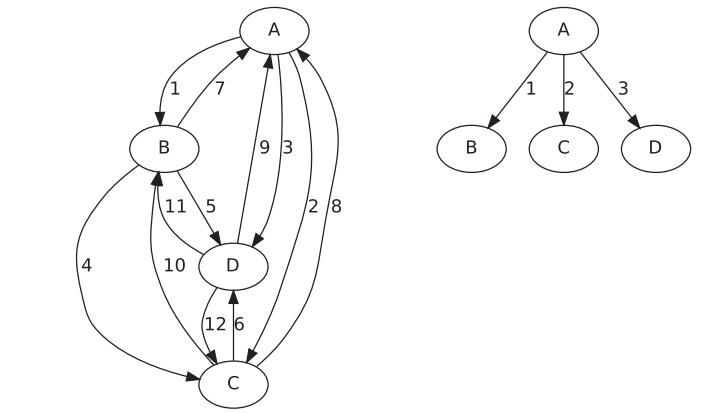
\includegraphics[width=12cm]{chaps/rw/digraph}}
	\caption{عنوانننننننننننننننننننننننننننننننننن}
	\label{fig:ch_rw:digraph}
\end{figure}



در ابتدا یال¬های گرف از طریق رابطه زیر وزن دهی می¬شود:

$-log zzzzzzzzzzzzzzzzzzz$

که در آن \lr{$(x \sim y)$ } رابطه بین جهش¬های \lr{x} و \lr{y} است و \lr{D} نمونه یا سمپل¬های موجود در داده است. بهترین درخت $\hat{T}$  از طریق کمینه¬کردن وزن¬های گراف بدست می¬آید.

\begin{math}
	y=xxxxxxxxxxxxxxxxxxxxxxxxxxx
\end{math}

در شکل بالا محتمل¬ترین \gls{phylogenytree} با بیشینه \gls{likelihood} بر اساس اطلاعات نمونه¬برداری شده بدست می¬آید. در این شکل گراف اولیه و درخت متناظر آن مشاهده می¬شود. مجموع همه وزن¬ها در درخت نهایی با شرط کمینه سازی برابر هفت است که این مقدار کمترین مقدار ممکن است. 


\subsection{پایگاه داده:}

در این مقاله از پایگاه داده تولی¬یابی تک سلولی هو¬ و همکاران \cite{hou2012single} استفاده شده است. این مجموع داده از توالی¬یابی تک¬سلولی \gls{dna} نمونه¬های توموری یک نوع خاص از \gls{thrombocythemia}جمع¬آوری شده است. این مجموعه داده شامل 58 سلول منفرد و 18 نوع جهش یکتا است. اطلاعات کامل در مورد این پایگاه داده از جمله، نام و نوع جهش¬های موجود در دیتابیس، نوع روش نمونه¬برداری و اطلاعاتی دیگر در پایگاه داده \lr{COSMIC} در دسرس عموم قرار دارد. ماتریس ژنوتایپی این پایگاه داده شامل سه مقدار صفر، یک و دو می¬باشد که در آن صفر بیانگر عدم وجود جهش،  یک بیانگر جهش هتروزیگوت و دو نمایانگر جهش هموزیگوت است. یکی از معایب این پایگاه داده نرخ بالای خطای توالی¬یابی تک¬سلولی و بالا¬ بودن نرخ داده¬های از دست رفته (در حدود 45 درصد کل داده¬ها) می¬باشد. همین امر سبب می¬شود تنوع \gls{phylogenytree} نسبت داده شده به این پایگاه داده زیاد باشد. در واقع با در نظر گرفتن حالت¬های مختلف روابط دو¬به¬دوی جهش¬های گوناگون، می¬توان درخت¬های جهشی متنوعی از داده¬ها استنباط کرد. 

\subsection{معیار ارزیابی: }






















